\documentclass[aspectratio=169]{beamer}
\usetheme{default}
\usecolortheme{dove}
\usefonttheme{serif}
\setbeamertemplate{navigation symbols}{}
\setbeamertemplate{footline}{}
\beamertemplatenavigationsymbolsempty

\usepackage{amsmath,amssymb}
\usepackage{graphicx}
\usepackage[most]{tcolorbox}

\graphicspath{{figs/}}

\definecolor{key}{rgb}{0.10,0.35,0.65}
\setbeamercolor{frametitle}{fg=key}

\title{SPF Stellarator Neutronics Meeting}
\author{Thaddaeus Kiker}
\date{\today}

\begin{document}

% 1. Title
\begin{frame}[plain]
  \titlepage
\end{frame}

% 2. Miscellaneous Updates
\begin{frame}{Miscellaneous Updates}
  \begin{itemize}
    \item Firefighters at my apartment again this past Sunday during the move
    \item 3D-printing saga for the HBT-H tokamak/stellarator-hybrid build
    \item APS abstract submission deadline is making things really hectic right now
  \end{itemize}
\end{frame}

% 2b. Notes screenshots grid (5x4), no title
\begin{frame}[plain]
  \centering
  \setlength{\tabcolsep}{1.5pt}\renewcommand{\arraystretch}{0.6}
  \begin{tabular}{ccccc}
    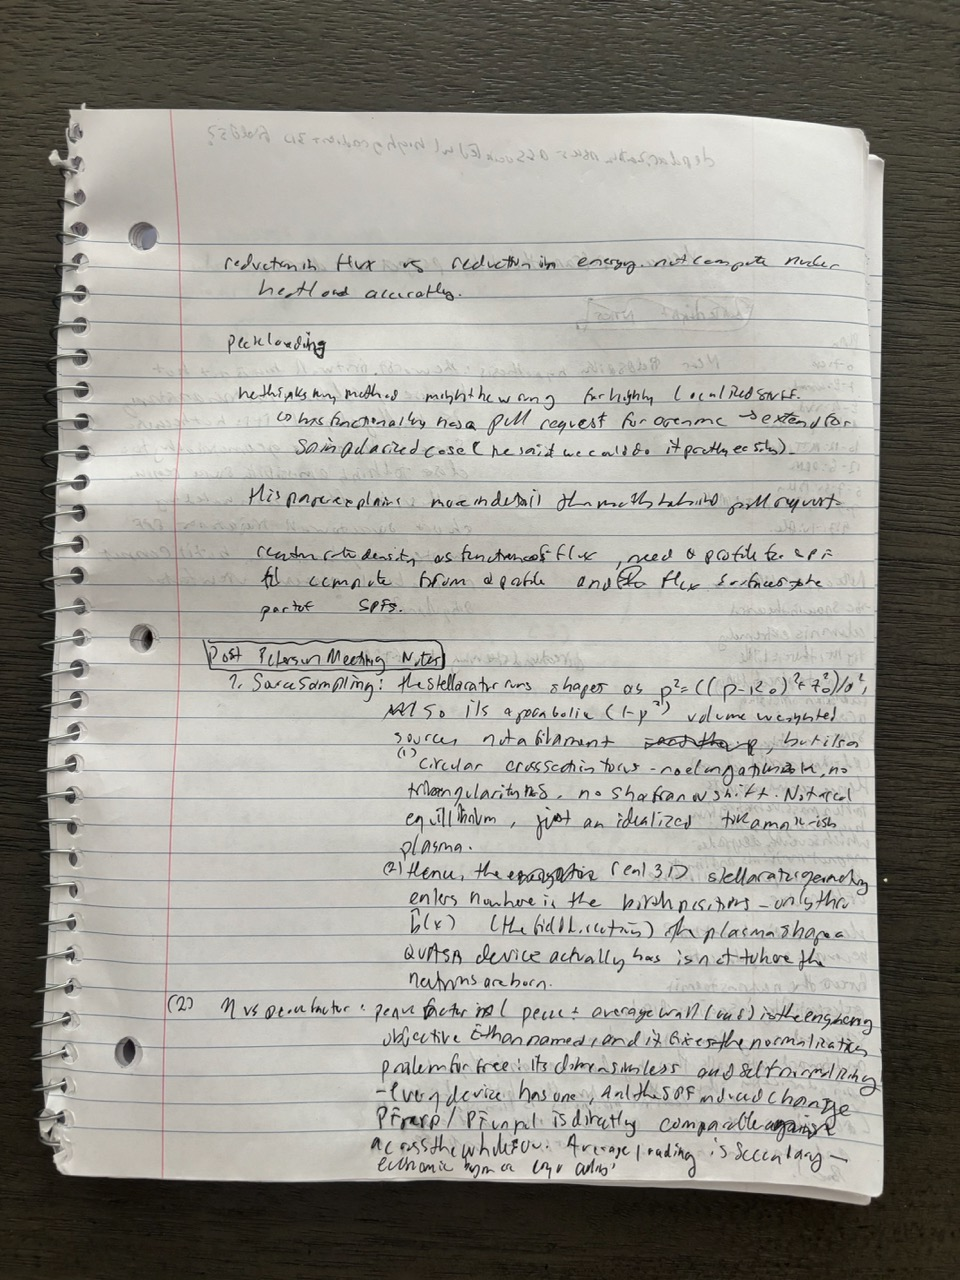
\includegraphics[width=.185\textwidth,height=.2\textheight,keepaspectratio]{notes/note01} & 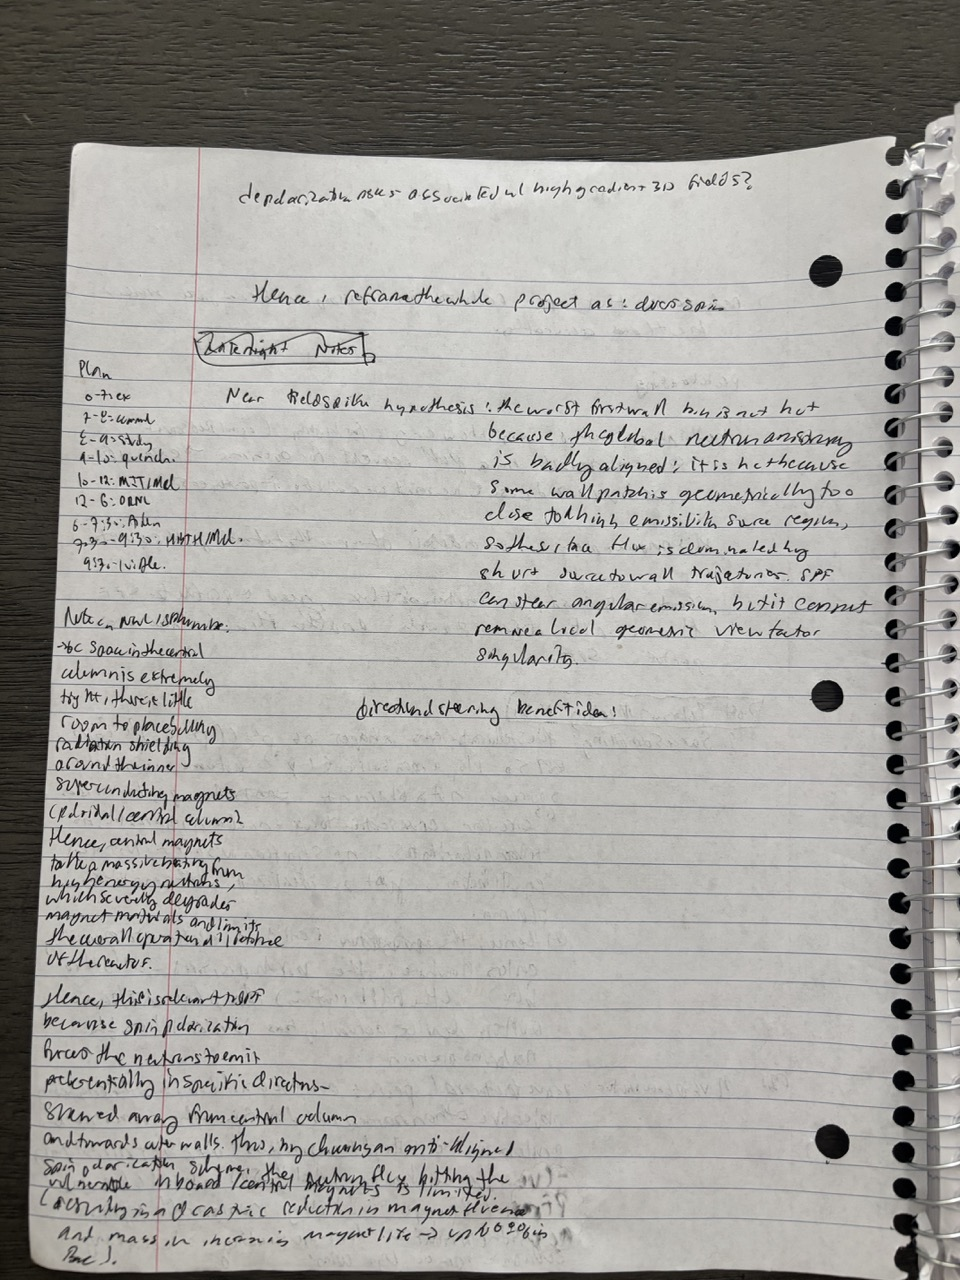
\includegraphics[width=.185\textwidth,height=.2\textheight,keepaspectratio]{notes/note02} & 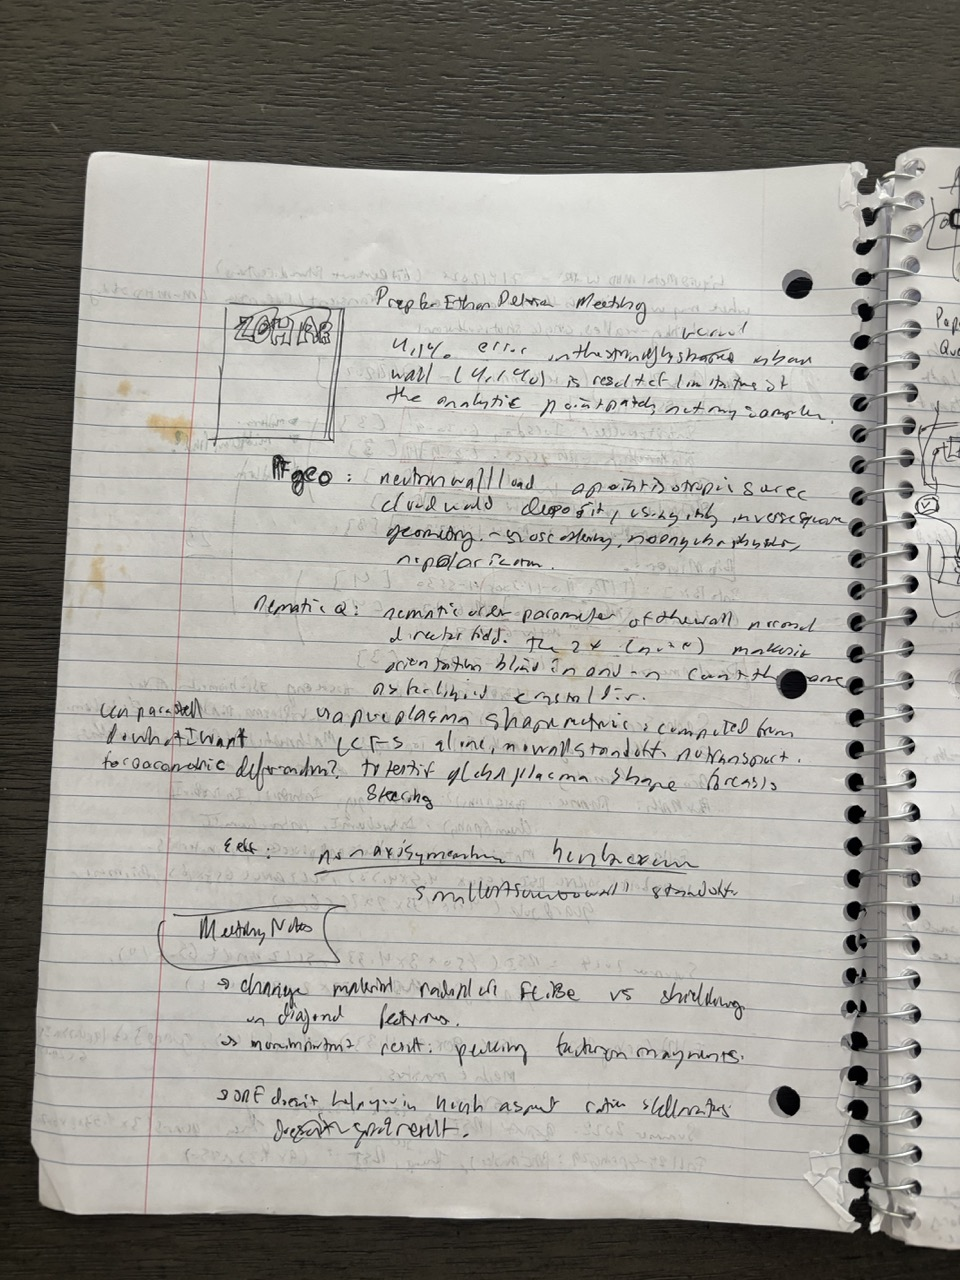
\includegraphics[width=.185\textwidth,height=.2\textheight,keepaspectratio]{notes/note03} & 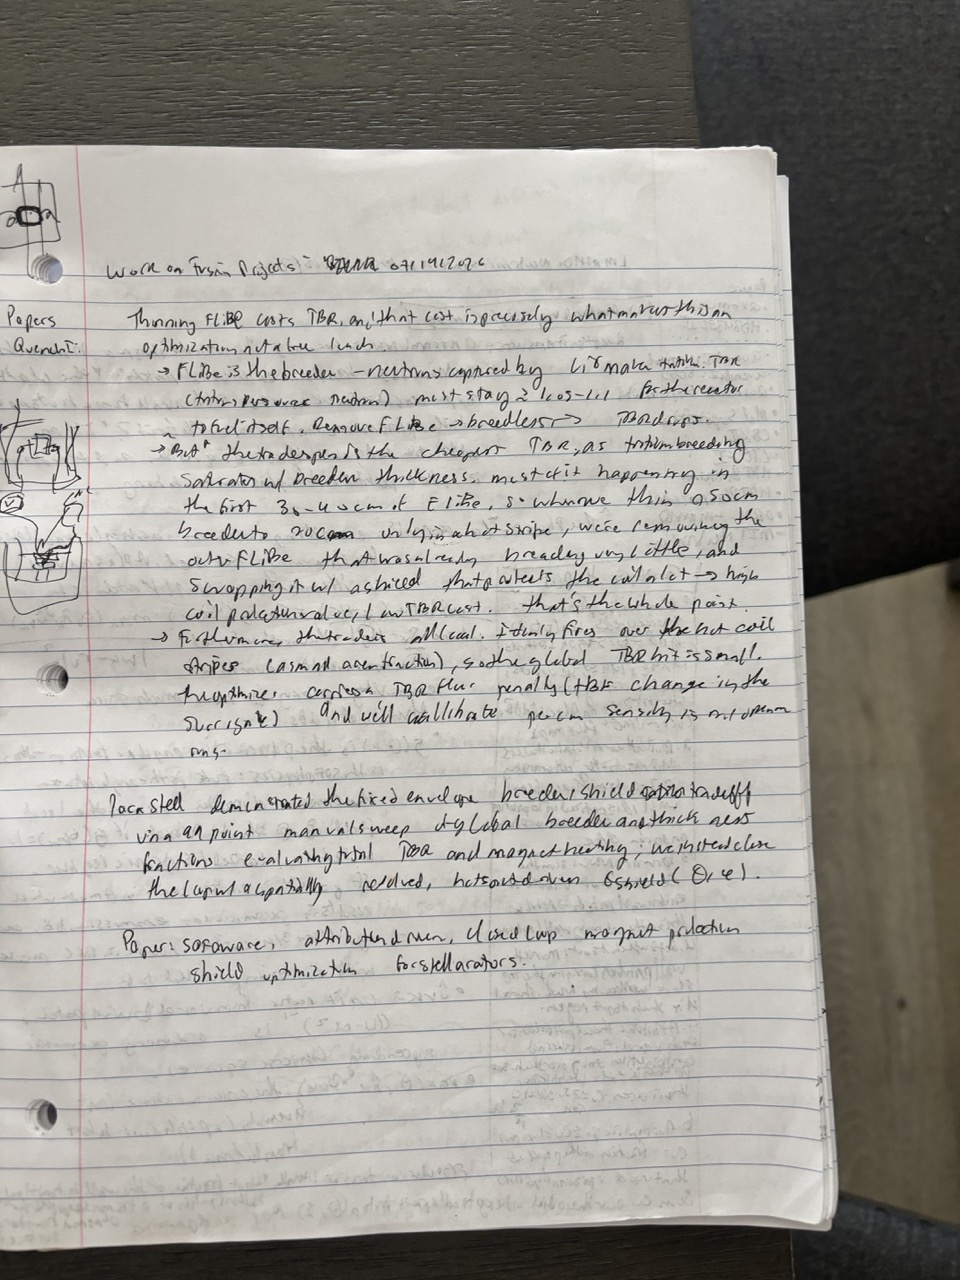
\includegraphics[width=.185\textwidth,height=.2\textheight,keepaspectratio]{notes/note04} & 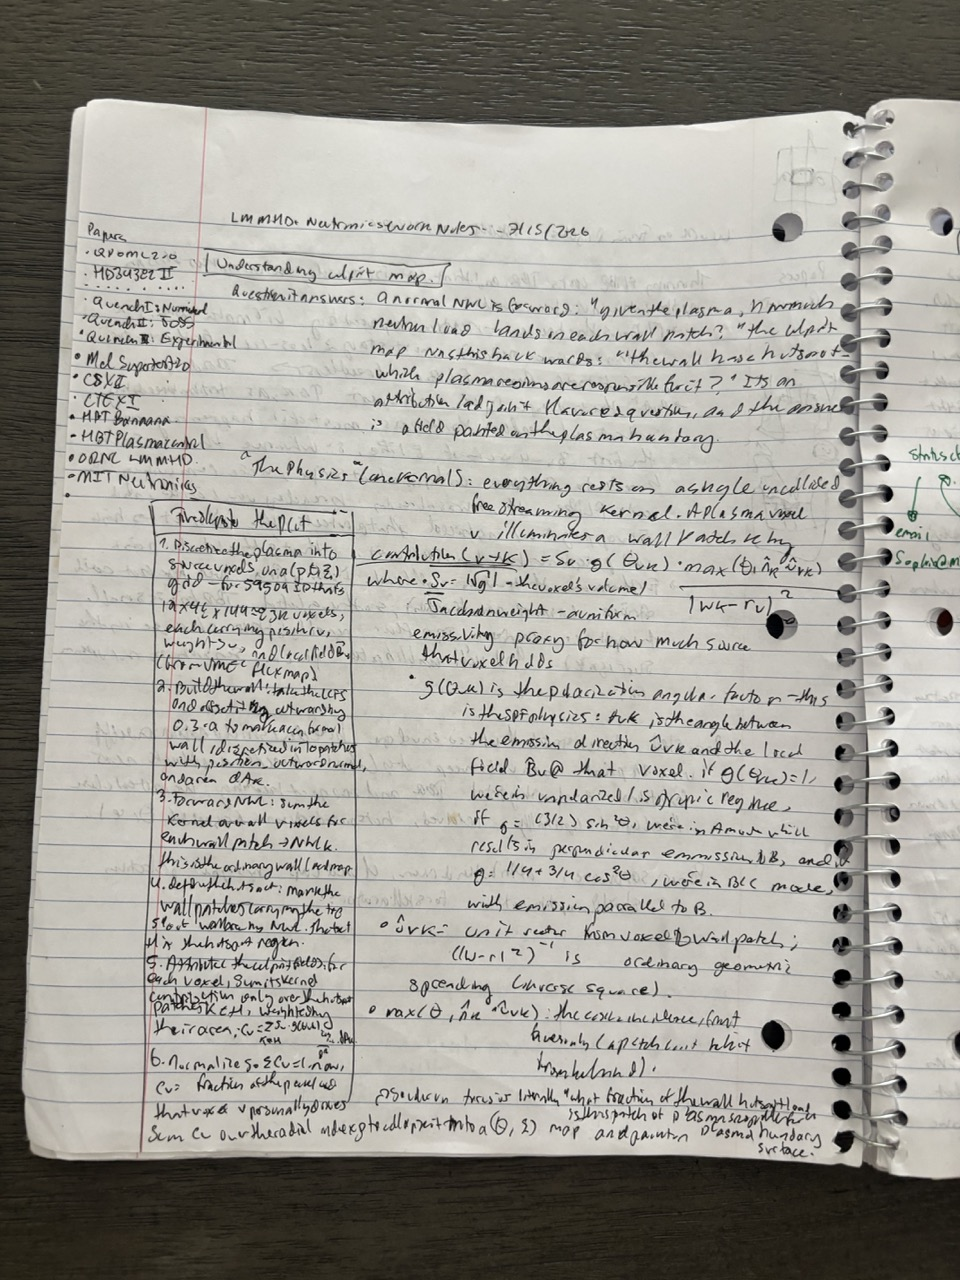
\includegraphics[width=.185\textwidth,height=.2\textheight,keepaspectratio]{notes/note05} \\
    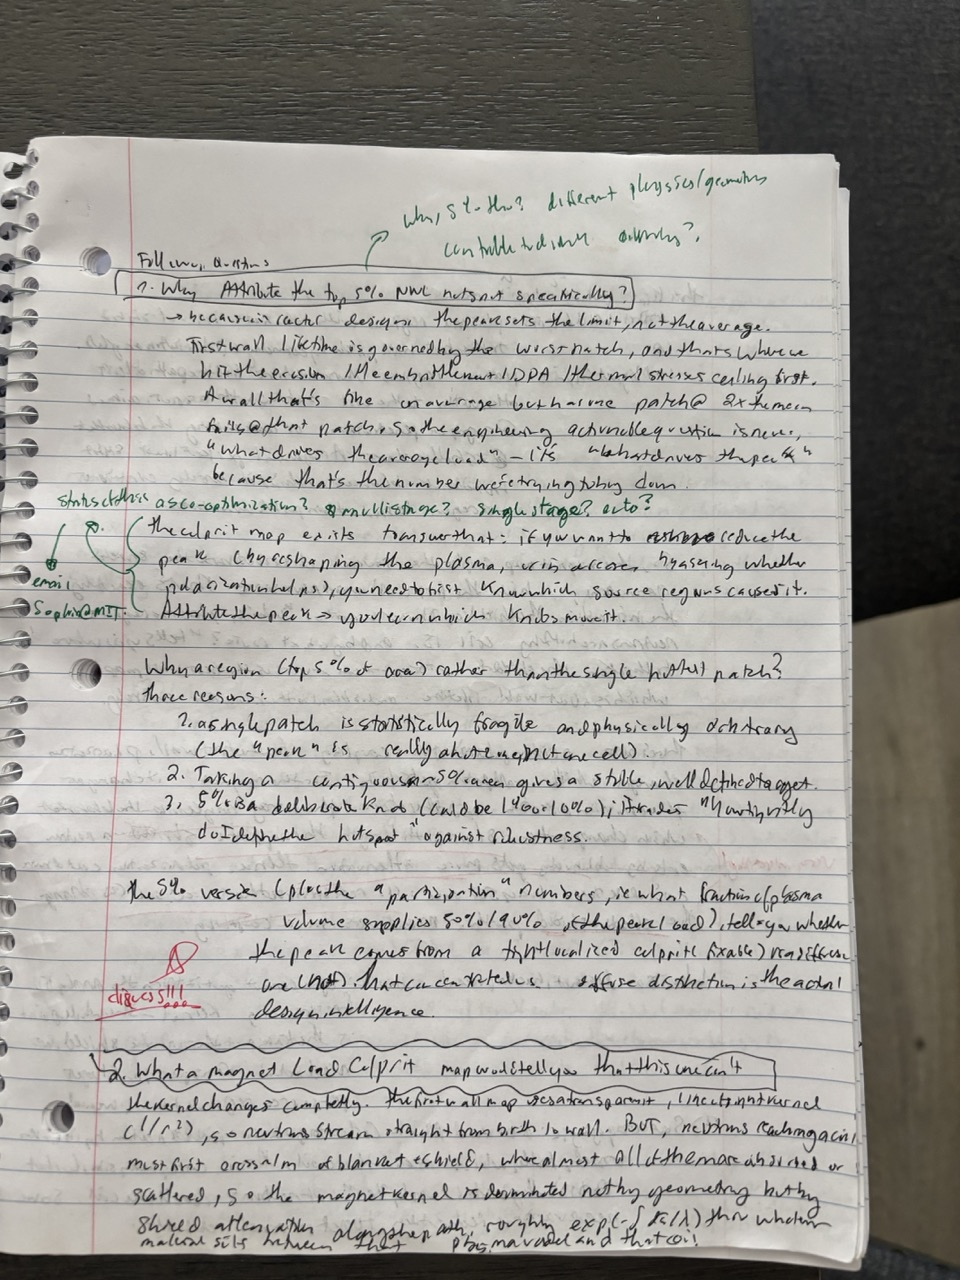
\includegraphics[width=.185\textwidth,height=.2\textheight,keepaspectratio]{notes/note06} & 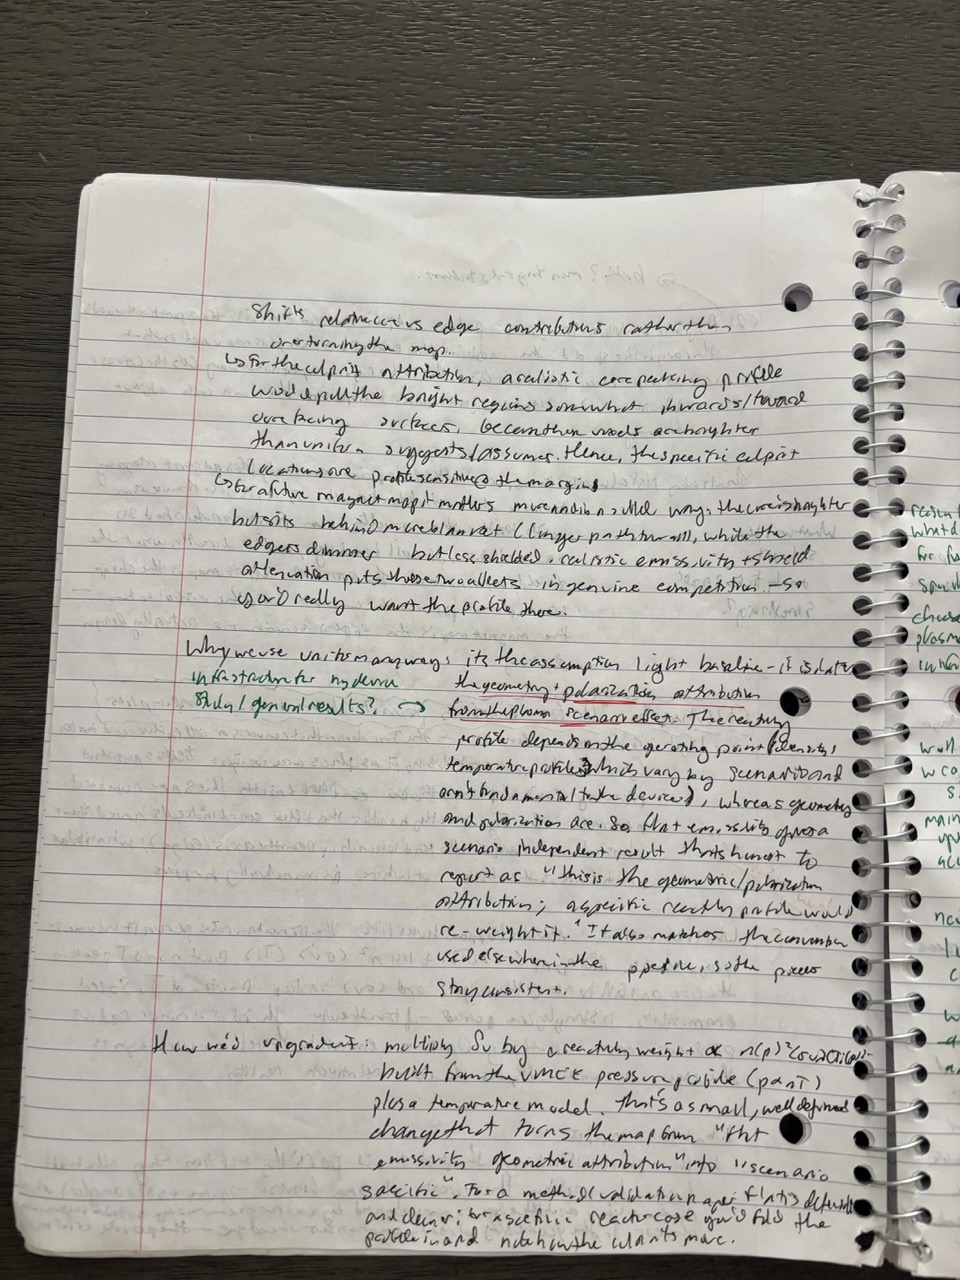
\includegraphics[width=.185\textwidth,height=.2\textheight,keepaspectratio]{notes/note07} & 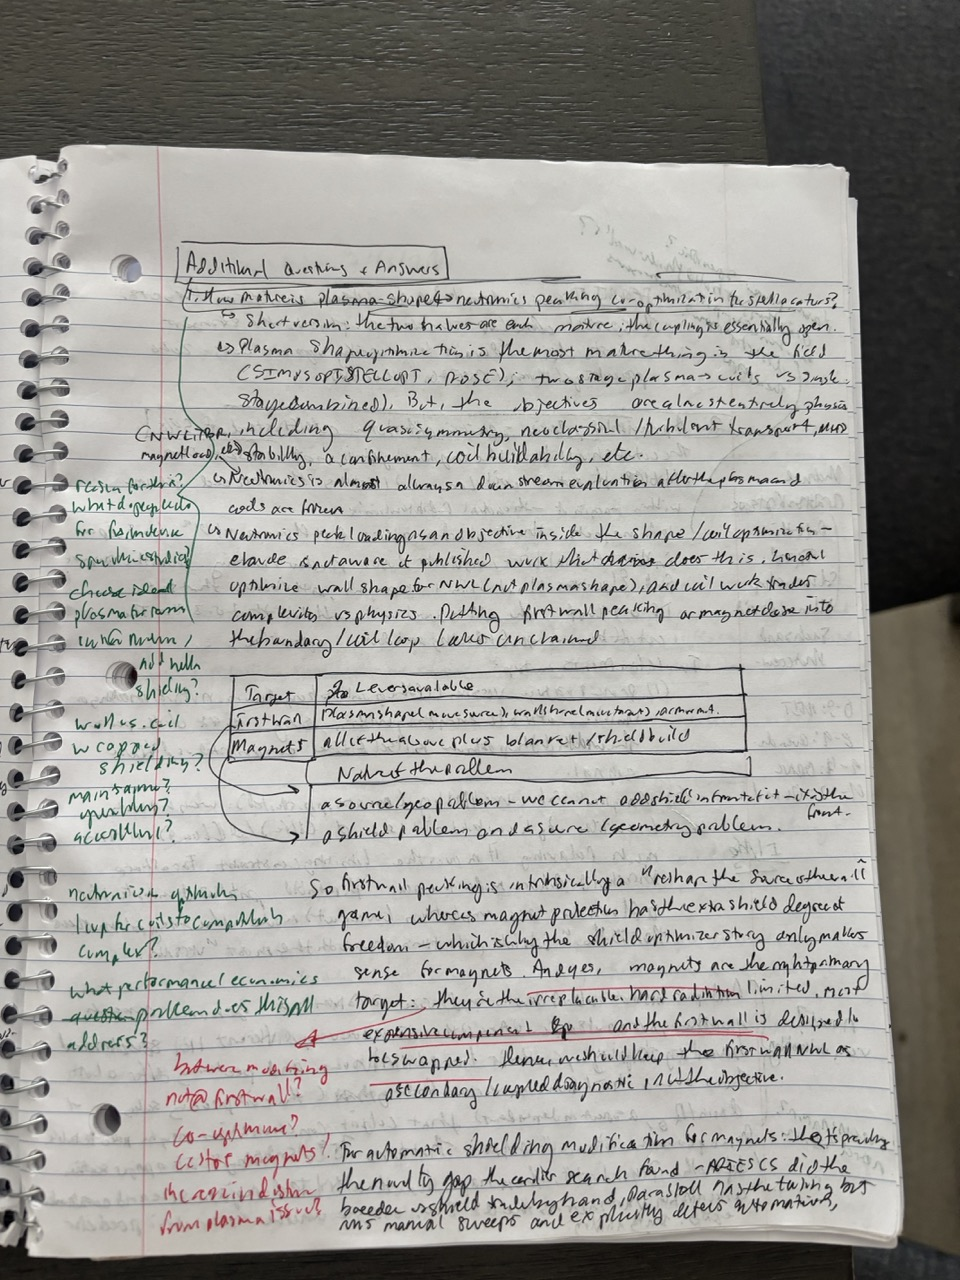
\includegraphics[width=.185\textwidth,height=.2\textheight,keepaspectratio]{notes/note08} & 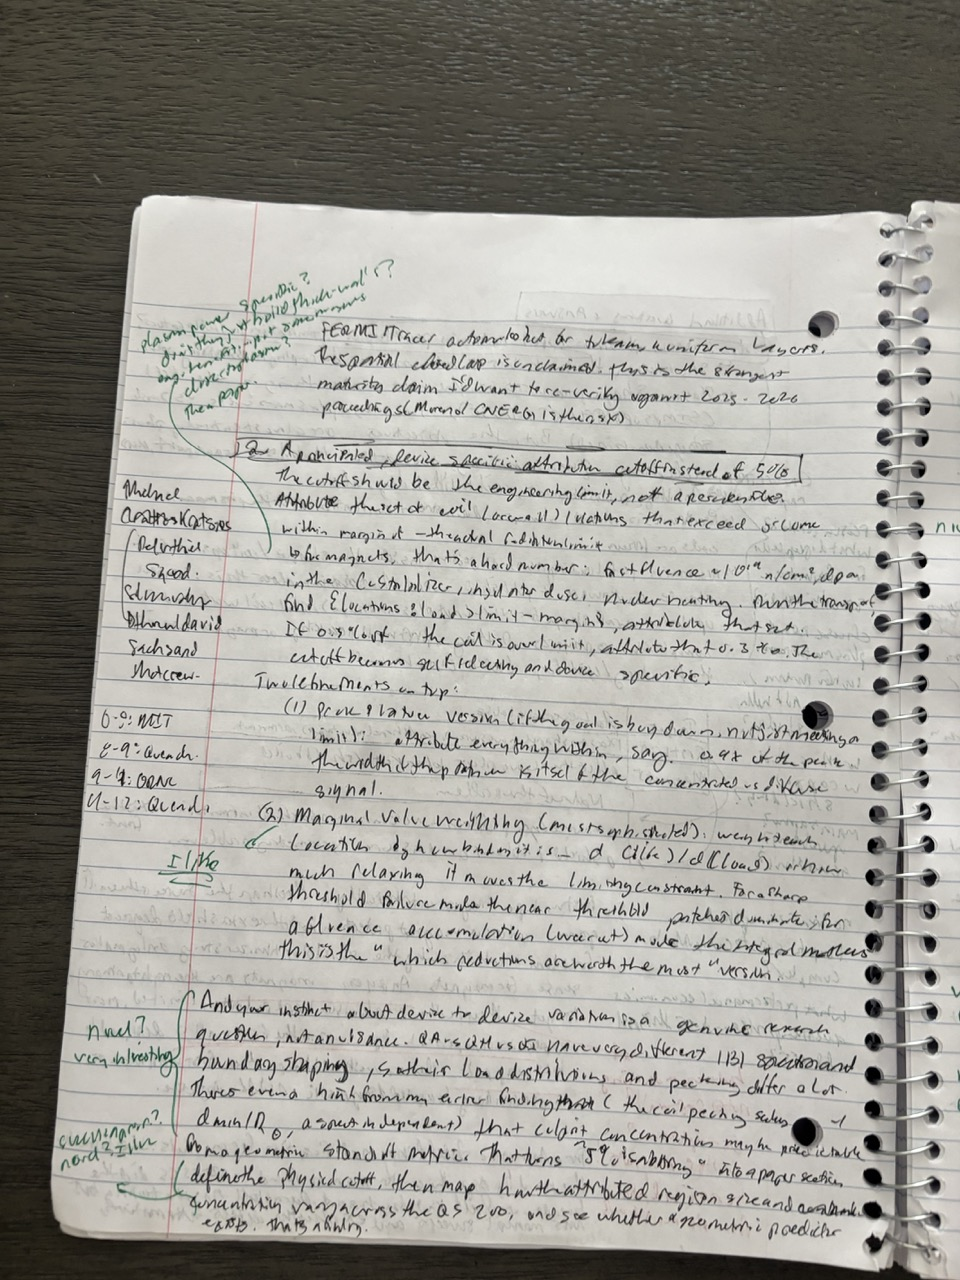
\includegraphics[width=.185\textwidth,height=.2\textheight,keepaspectratio]{notes/note09} & 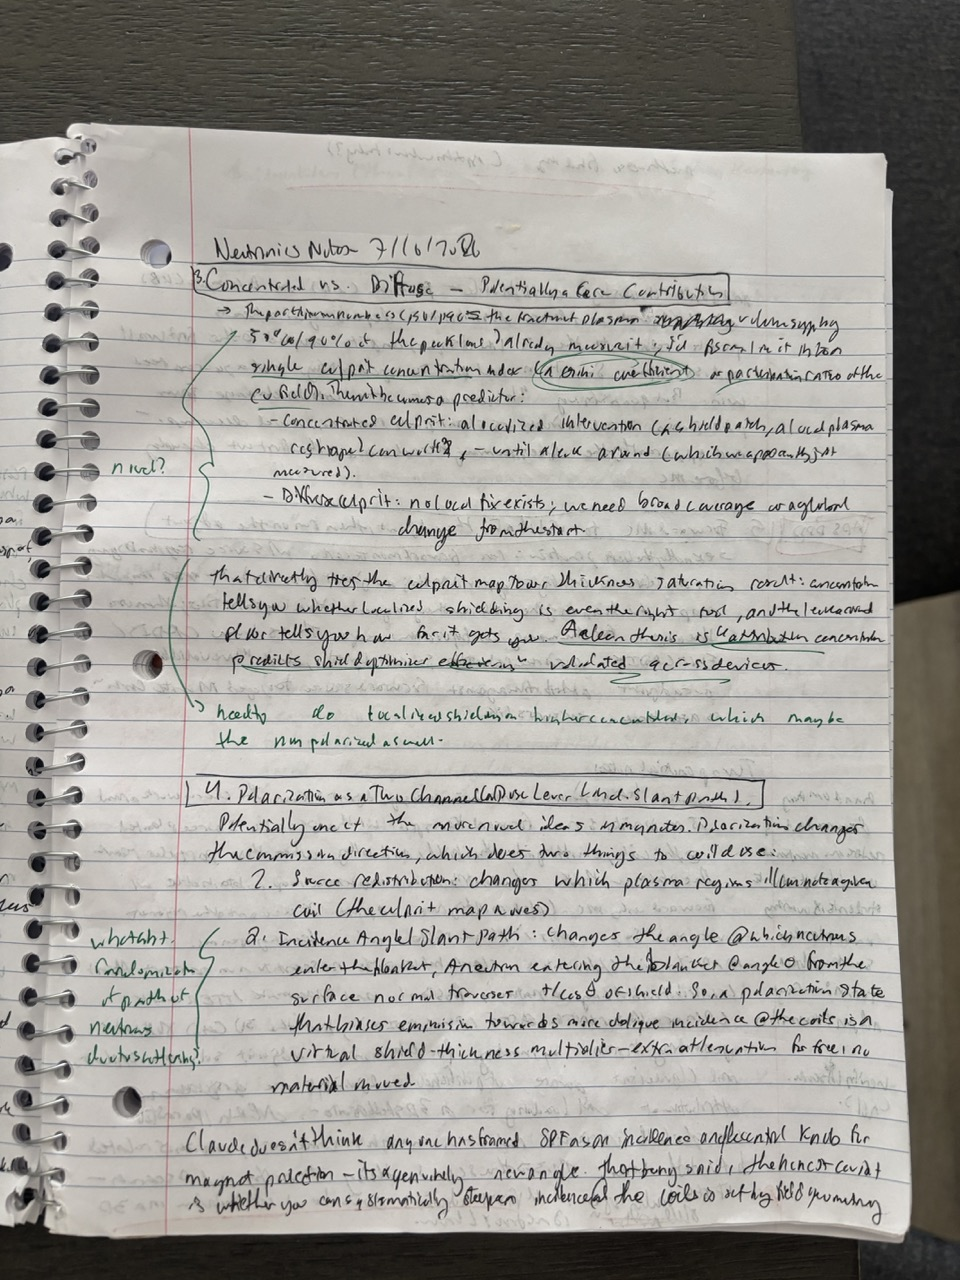
\includegraphics[width=.185\textwidth,height=.2\textheight,keepaspectratio]{notes/note10} \\
    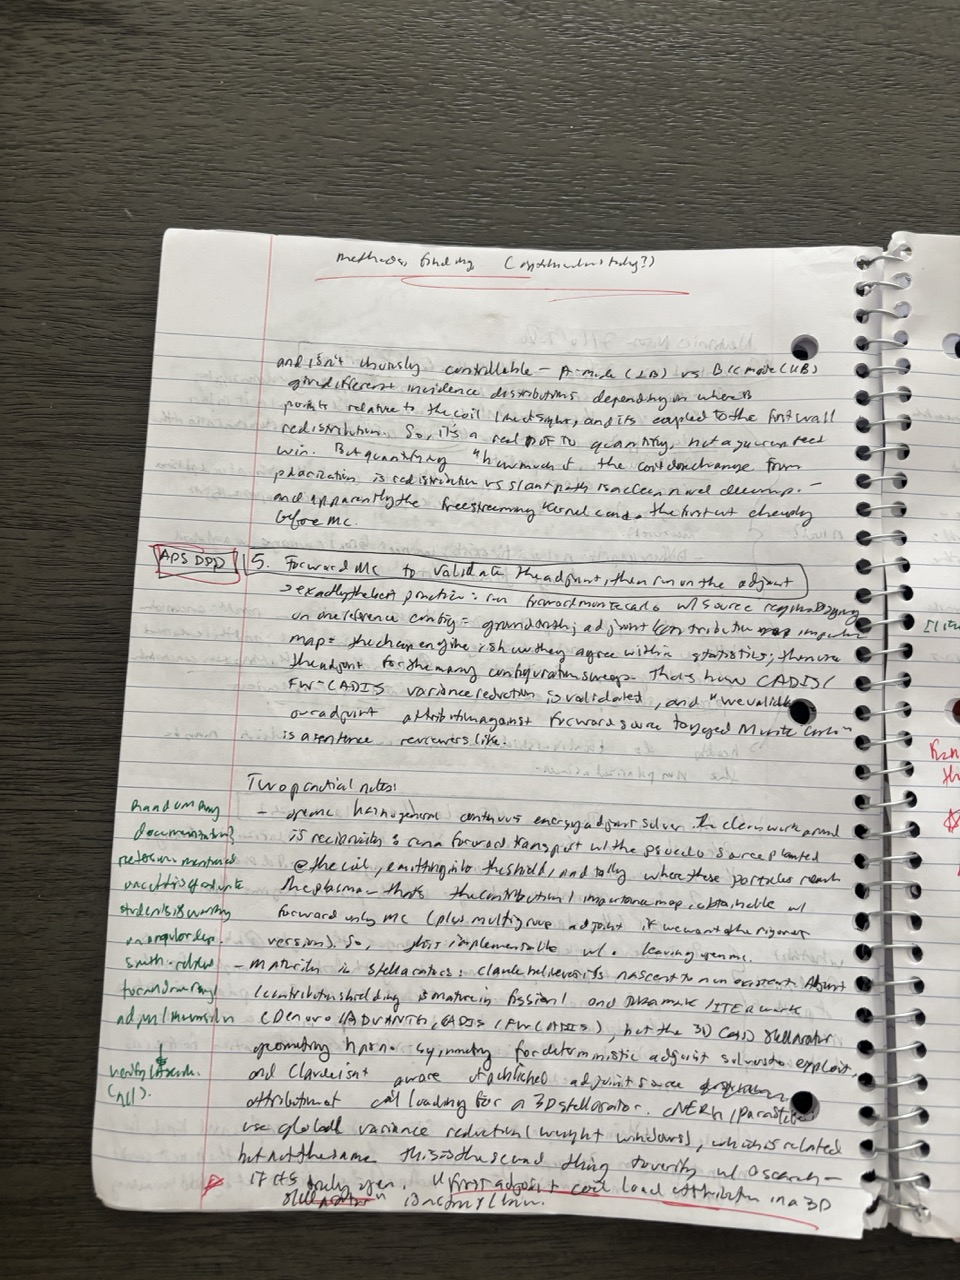
\includegraphics[width=.185\textwidth,height=.2\textheight,keepaspectratio]{notes/note11} & 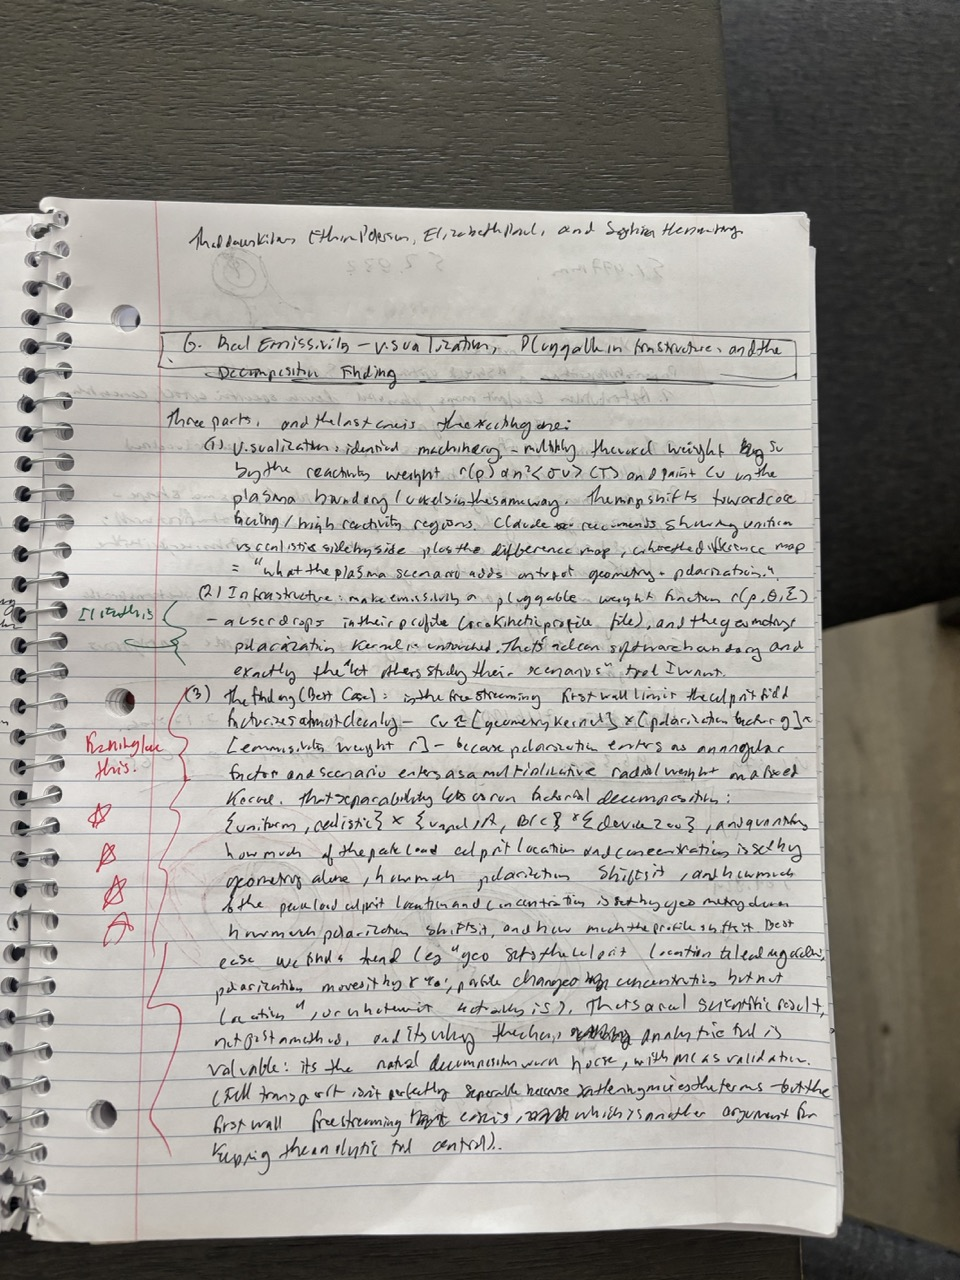
\includegraphics[width=.185\textwidth,height=.2\textheight,keepaspectratio]{notes/note12} & 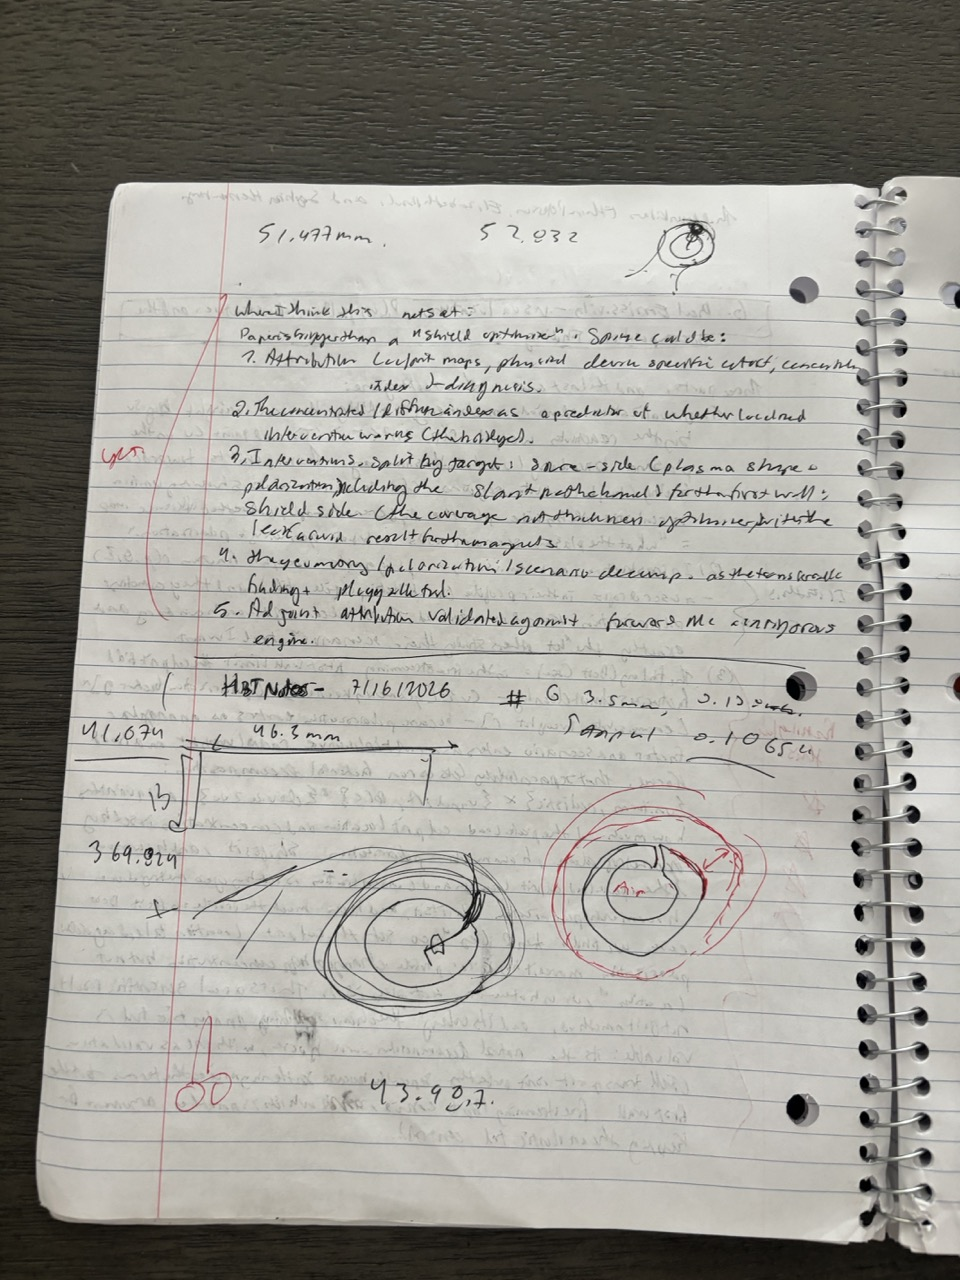
\includegraphics[width=.185\textwidth,height=.2\textheight,keepaspectratio]{notes/note13} & 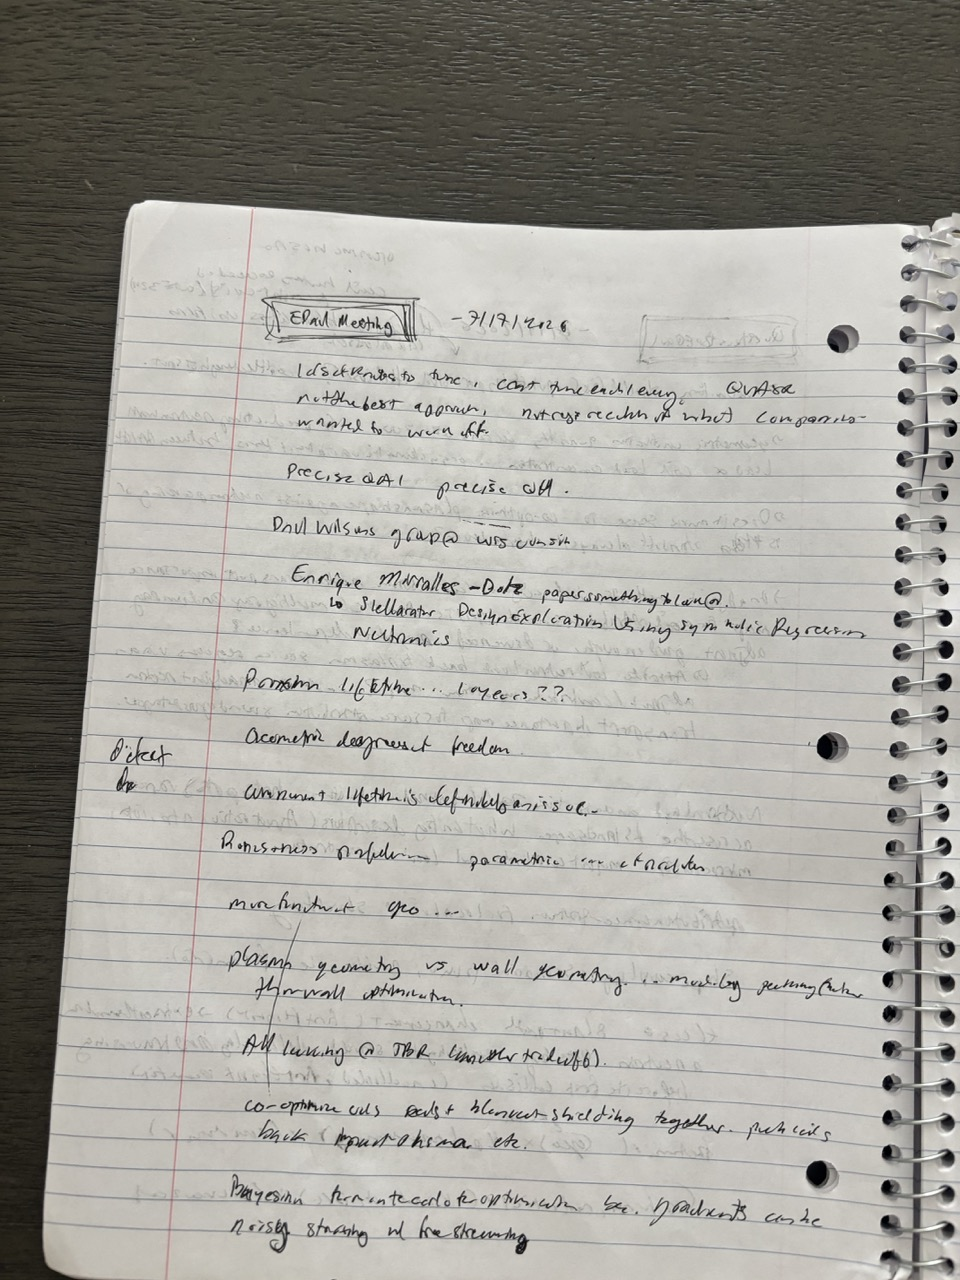
\includegraphics[width=.185\textwidth,height=.2\textheight,keepaspectratio]{notes/note14} & 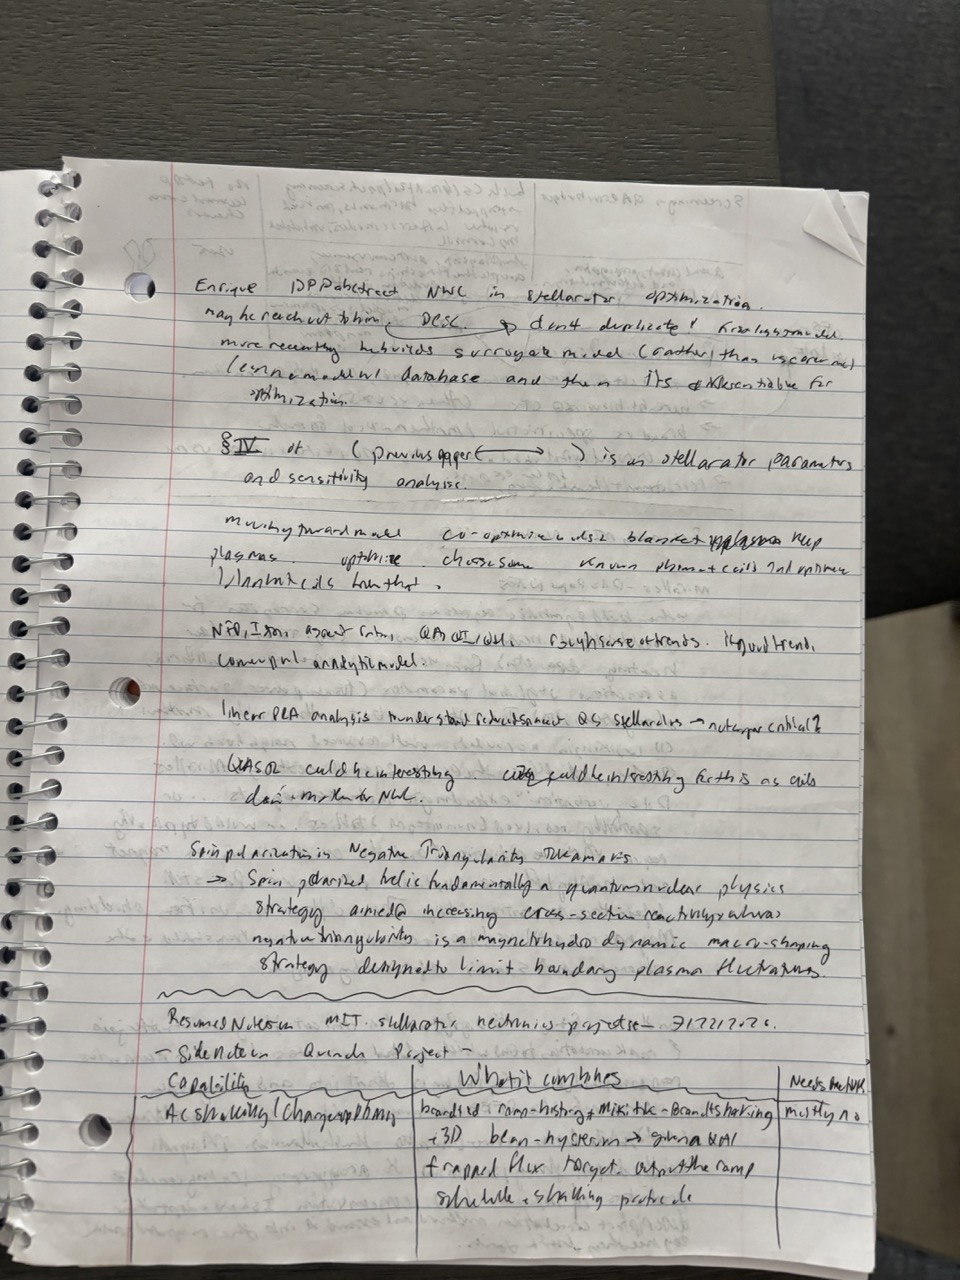
\includegraphics[width=.185\textwidth,height=.2\textheight,keepaspectratio]{notes/note15} \\
    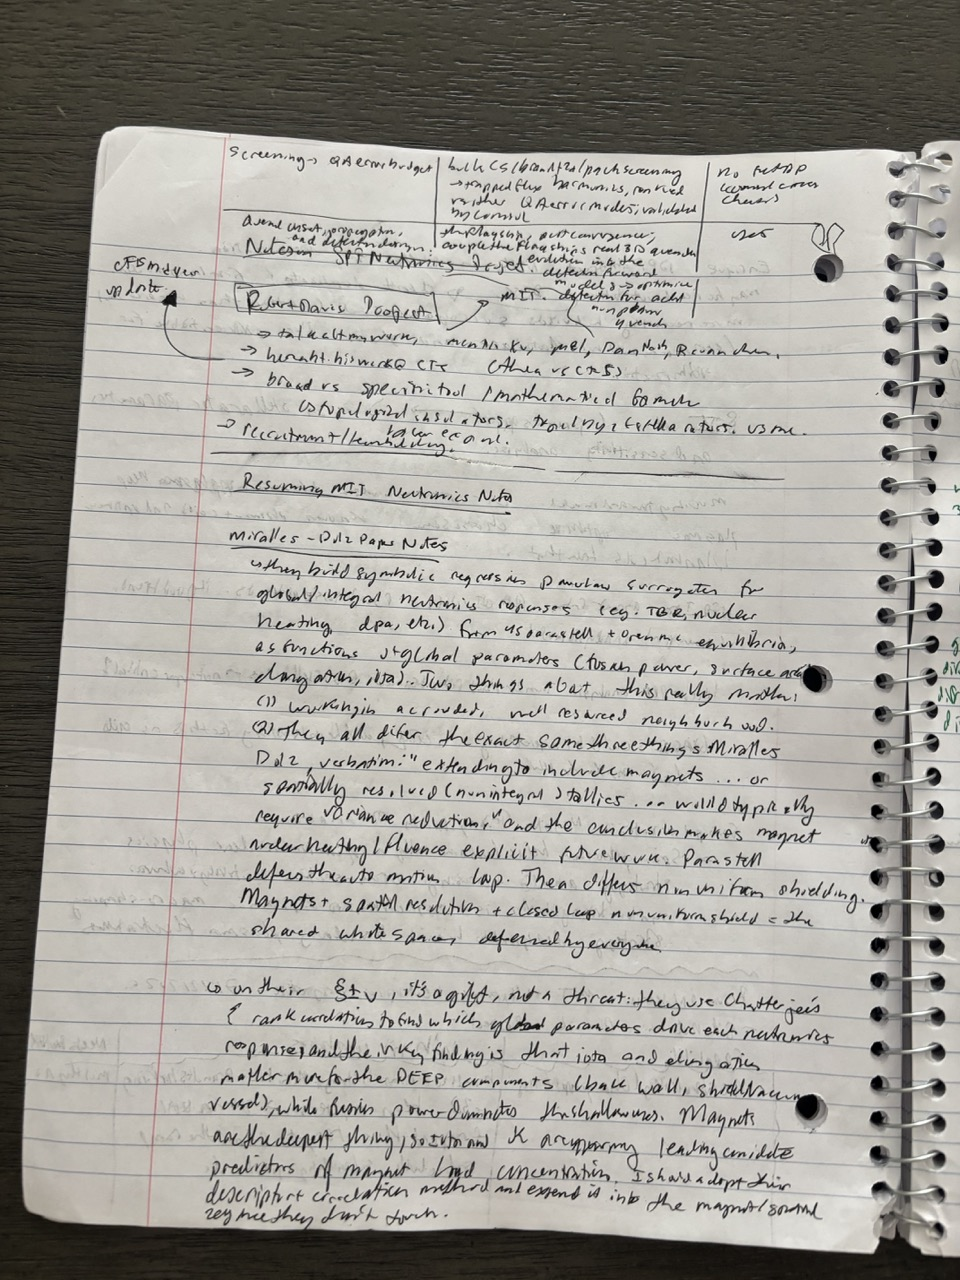
\includegraphics[width=.185\textwidth,height=.2\textheight,keepaspectratio]{notes/note16} & 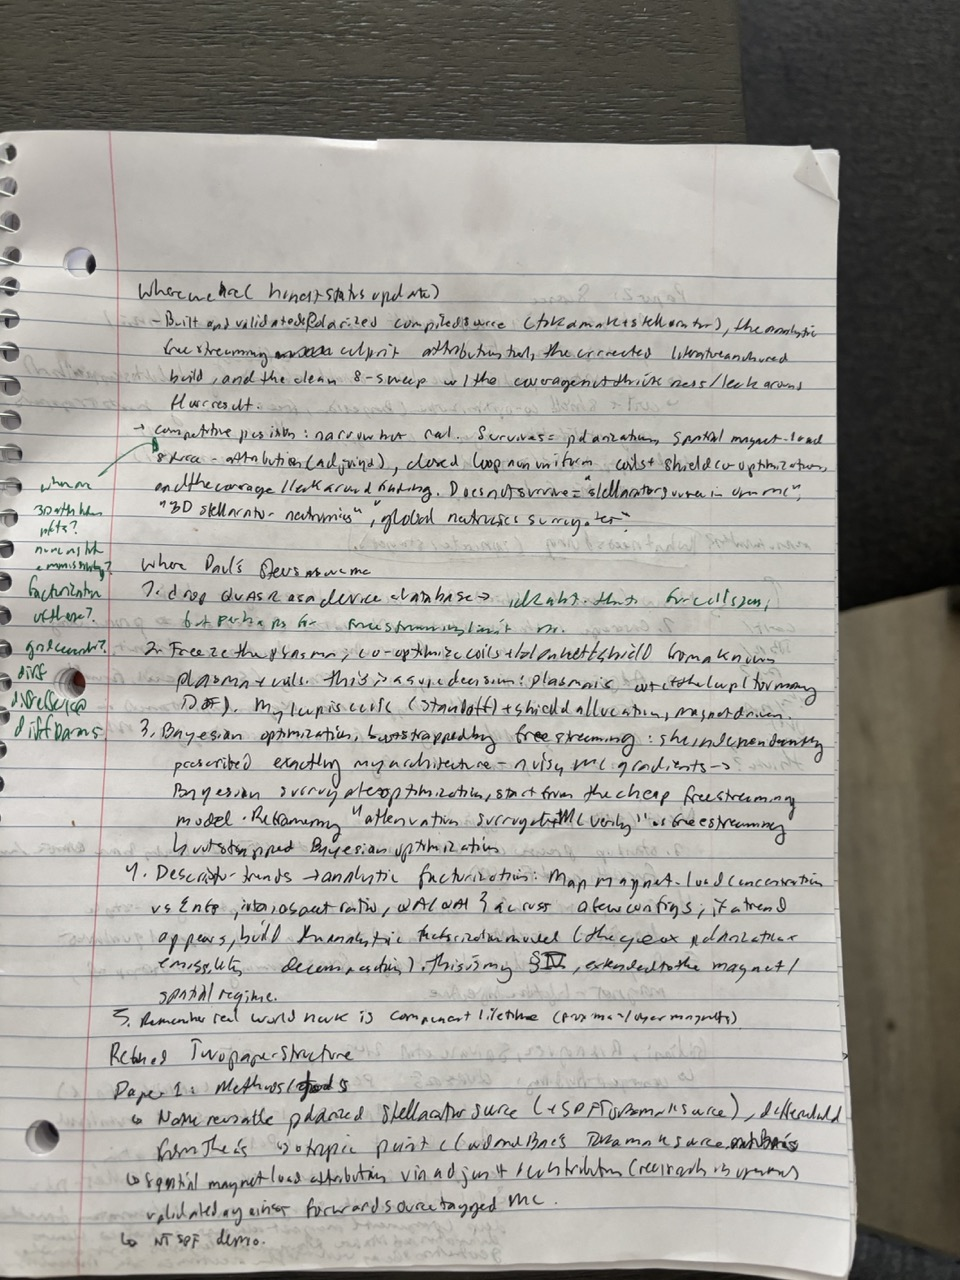
\includegraphics[width=.185\textwidth,height=.2\textheight,keepaspectratio]{notes/note17} & 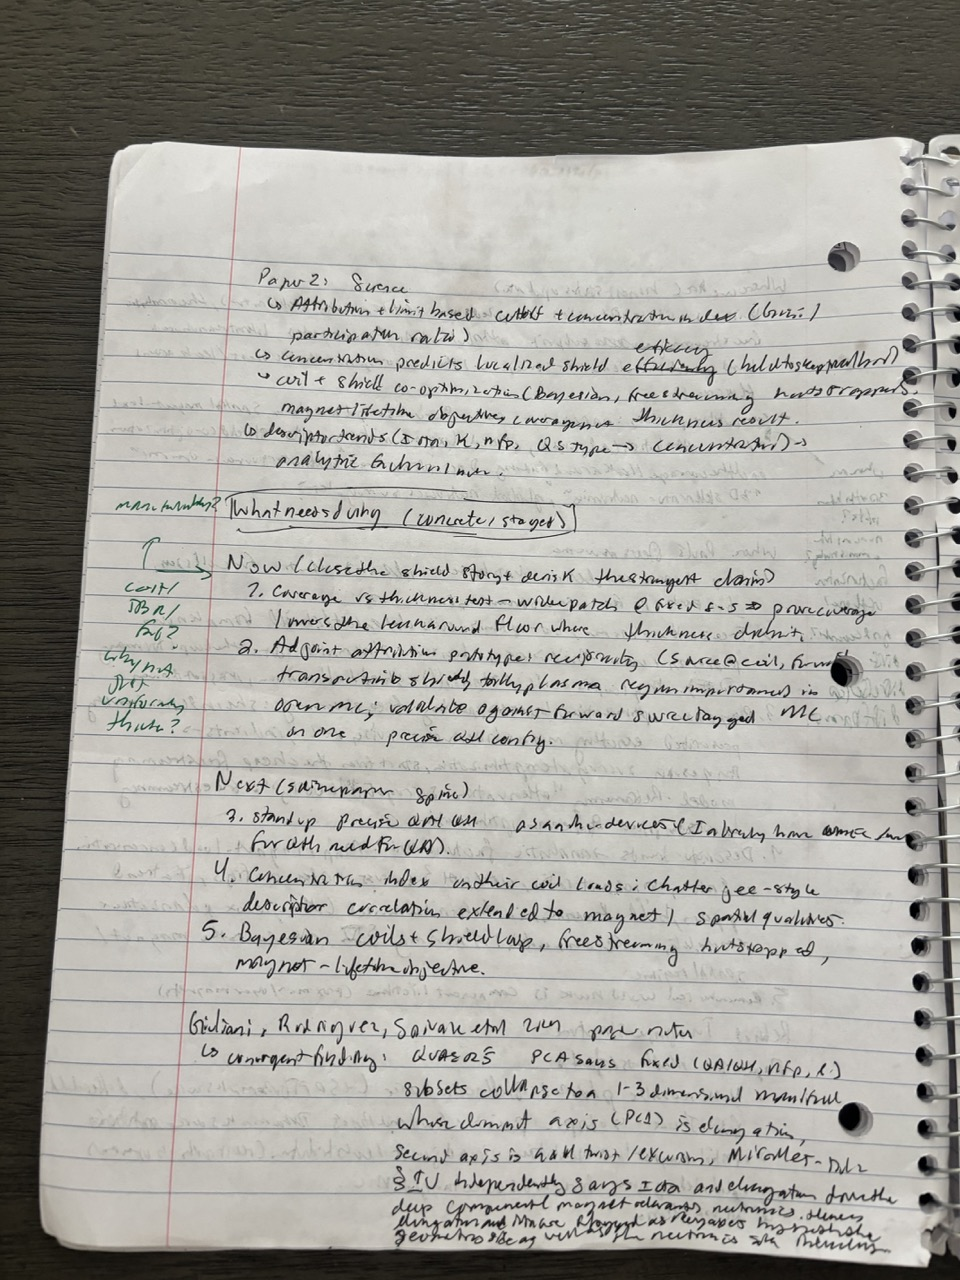
\includegraphics[width=.185\textwidth,height=.2\textheight,keepaspectratio]{notes/note18} & 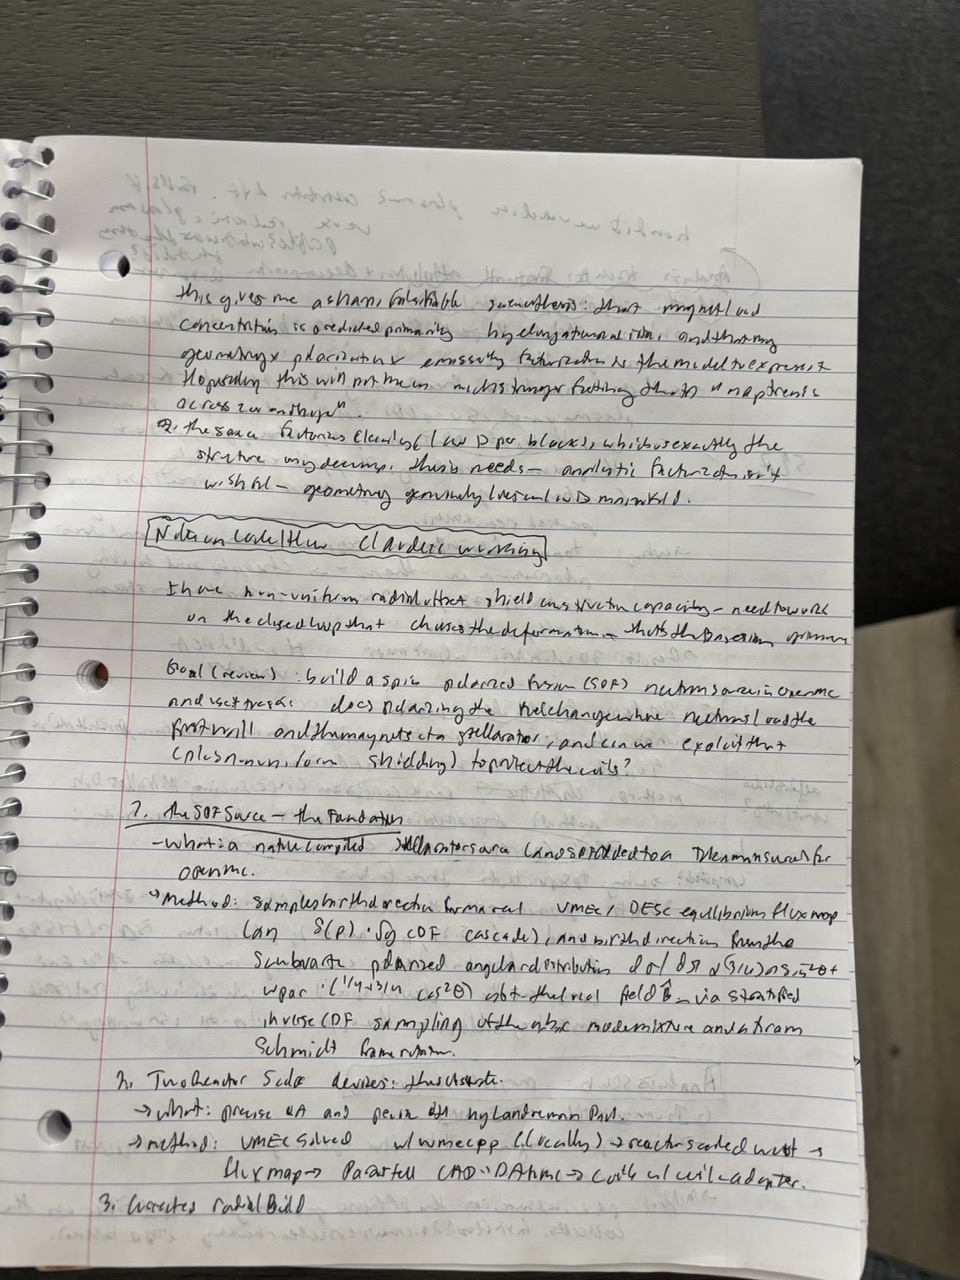
\includegraphics[width=.185\textwidth,height=.2\textheight,keepaspectratio]{notes/note19} & 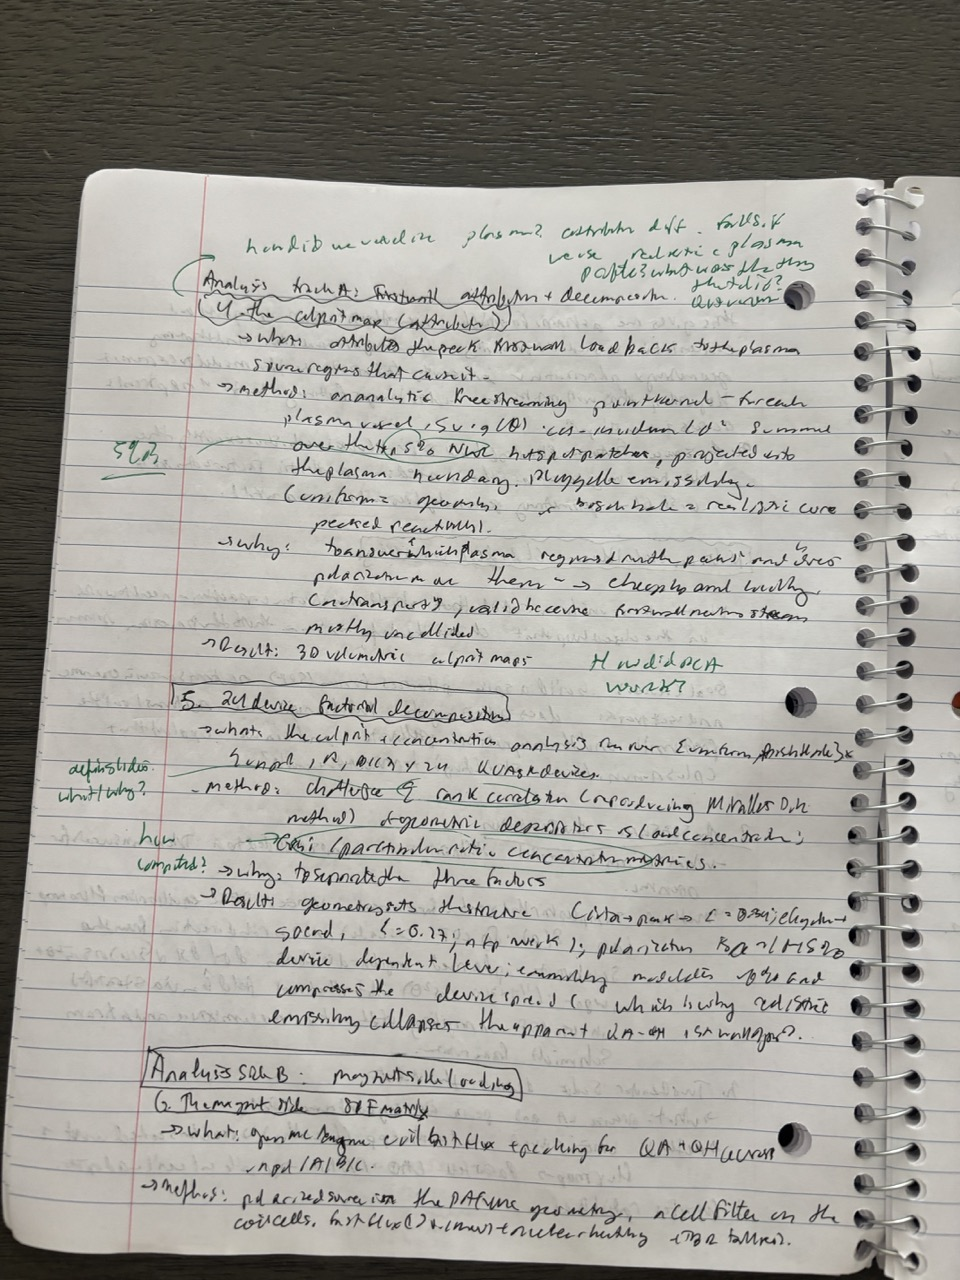
\includegraphics[width=.185\textwidth,height=.2\textheight,keepaspectratio]{notes/note20} \\
  \end{tabular}
\end{frame}

% 3. Elizabeth Paul image, no title
\begin{frame}[plain]
  \begin{center}
    \includegraphics[height=0.85\textheight]{elizabeth-paul.jpg}
  \end{center}
\end{frame}

% 4. Miralles paper
\begin{frame}[plain]
  \begin{center}
    \includegraphics[height=0.9\textheight]{paper_miralles.png}
  \end{center}
\end{frame}

% 5. Helios paper
\begin{frame}[plain]
  \begin{center}
    \includegraphics[height=0.9\textheight]{paper_helios.png}
  \end{center}
\end{frame}

% 6. ParaStell paper
\begin{frame}[plain]
  \begin{center}
    \includegraphics[height=0.9\textheight]{paper_parastell.png}
  \end{center}
\end{frame}

% 7. PCA paper
\begin{frame}[plain]
  \begin{center}
    \includegraphics[height=0.9\textheight]{paper_pca.png}
  \end{center}
\end{frame}

% 8. Work Summary
\begin{frame}{Work Summary}
  \begin{itemize}
    \item First-wall attribution and decomposition
    \item Magnet-side loading
    \item Non-uniform shield design via a Bayesian loop
    \item Coverage vs.\ thickness vs.\ placement
    \item Need for adjoint coil attribution
  \end{itemize}
\end{frame}

% 9. First-Wall Attribution: The Point-Kernel
\begin{frame}{First-Wall Attribution: The Point-Kernel}
  \footnotesize
  Forward uncollided wall load on patch $k$:
  \[
    \mathrm{NWL}_k = \sum_{v} S_v\, g(\theta_{vk})\,
      \frac{\max(0,\ \hat{n}_k\cdot\hat{u}_{vk})}{|\mathbf{w}_k-\mathbf{r}_v|^2}
  \]
  Culprit field (attribution), restricted to hot-spot patches $H$:
  \[
    C_v = \sum_{k\in H} S_v\, g(\theta_{vk})\,
      \frac{\max(0,\ \hat{n}_k\cdot\hat{u}_{vk})}{|\mathbf{w}_k-\mathbf{r}_v|^2}\, dA_k
  \]
  Gini coefficient of the loading distribution:
  \[
    G = \frac{\sum_i \sum_j |x_i - x_j|}{2\, n^2\, \bar{x}}
  \]
  \begin{itemize}
    \item Angular factor $g$: $1$ (unpolarized), $\tfrac{3}{2}\sin^2\theta$
      (A, $\perp B$), or $\tfrac{1}{4}+\tfrac{3}{4}\cos^2\theta$ (B/C, $\parallel B$);
      $\theta$ = angle between emission direction and local $B$.
  \end{itemize}
\end{frame}

% 9b. First-Wall Attribution and Decomposition
\begin{frame}{First-Wall Attribution and Decomposition}
  \footnotesize
  \begin{itemize}
    \item Decomposition across twenty-four devices, factorial
      \{uniform, Bosch--Hale emissivity\} $\times$ \{unpolarized, A, B/C\}:
      geometry sets the structure ($\iota\!\to\!$ peak; elongation $\to$ spread),
      polarization is a $\sim$10--15\% device-dependent lever, emissivity
      $\sim$6\% and compresses the device spread.
    \item Under uniform emissivity the QA-vs-QH peaking gap is large; but under
      realistic (core-peaked Bosch--Hale) the gap largely collapses.
  \end{itemize}
  \begin{tcolorbox}[colback=key!5,colframe=key!60,boxsep=2pt,left=4pt,right=4pt,top=2pt,bottom=2pt]
    \small
    Chatterjee rank-correlation coefficient:
    \[
      \xi_n(X,Y) = 1 - \frac{3\sum_{i=1}^{n-1}|r_{i+1}-r_i|}{n^2-1}
    \]
    Rank-based; $0$ = independent, $\to 1$ = $Y$ is a function of $X$; catches
    nonlinear/nonmonotonic dependence. Adopted from Miralles-Dolz's neutronics
    sensitivity analysis.
  \end{tcolorbox}
\end{frame}

% 9c. Chatterjee xi heatmap
\begin{frame}{Chatterjee $\xi$: What Drives the Wall Load}
  \begin{columns}[c]
    \begin{column}{0.62\textwidth}
      \includegraphics[width=\textwidth]{zoo_descriptor_xi.png}
    \end{column}
    \begin{column}{0.38\textwidth}
      \footnotesize
      \begin{itemize}
        \item $n=83$ configurations, free-streaming wall-load responses.
        \item Elongation $\to$ load concentration: $\xi=0.96$
          (shape anisotropy $0.83$) --- the poloidal shaping sets how
          peaked the wall load is.
        \item Aspect ratio and field-period count are comparatively weak levers.
        \item The polarization levers (perp./par.) are near-independent of these
          geometry descriptors --- polarization is a separate knob.
      \end{itemize}
    \end{column}
  \end{columns}
\end{frame}

% 9b. Decomposition figure on its own frame
\begin{frame}{Decomposition: Geometry Sets Structure}
  \begin{center}
    \includegraphics[width=0.68\textwidth]{decomp_iota_peak.png}
  \end{center}
\end{frame}

% 9d. Device renders — precise QA (wireframe, then coils) and precise QH
\begin{frame}{Precise QA Reactor}
  \begin{center}
    \includegraphics[height=0.9\textheight]{render_qa_wire.png}
  \end{center}
\end{frame}

\begin{frame}{Precise QA Reactor: Coils}
  \begin{center}
    \includegraphics[height=0.9\textheight]{render_qa_coils.png}
  \end{center}
\end{frame}

\begin{frame}{Precise QH Reactor}
  \begin{center}
    \includegraphics[height=0.9\textheight]{render_qh_wire.png}
  \end{center}
\end{frame}

\begin{frame}{Precise QH Reactor: Coils}
  \begin{center}
    \includegraphics[height=0.9\textheight]{render_qh_coils.png}
  \end{center}
\end{frame}

% 10. Magnet-Side Loading
\begin{frame}{Magnet-Side Loading}
  \small
  \begin{columns}[T]
    \begin{column}{0.54\textwidth}
      \begin{itemize}
        \item Coil fast-flux + peaking for QA and QH, all polarization modes,
          identical radial build.
        \item Parallel-emission (B/C) polarization flattens QA magnet peaking
          $\sim$17\% and cuts flux $\sim$15\% (beneficial); QH only $\sim$3\%
          $\to$ spin polarization is a device-dependent magnet-protection lever.
        \item Caveat: the raw QA-vs-QH magnet flux gap is a coil-standoff effect
          (QA coils sit $\sim$1.9$\times$ further from the plasma), not a
          quasisymmetry-type advantage; the polarization result is a
          within-device comparison and is unaffected.
      \end{itemize}
    \end{column}
    \begin{column}{0.46\textwidth}
      \includegraphics[width=\textwidth]{magnet_polarization_matrix.png}\\[2pt]
      \includegraphics[width=\textwidth]{standoff_qa_qh.png}
    \end{column}
  \end{columns}
\end{frame}

% 11. Non-Uniform Shield Design and Placement
\begin{frame}{Non-Uniform Shield Design and Placement}
  \small
  \begin{itemize}
    \item Closed-loop non-uniform shield: a smooth Fourier thickness field
      $\delta(\theta,\phi)$ under a fixed-envelope breeder $\leftrightarrow$
      shield trade (coils fixed); Bayesian optimization with scikit-optimize
      (Gaussian-process \texttt{gp\_minimize}, since MC gradients are too noisy),
      bootstrapped by the cheap free-streaming model.
    \item Coverage vs.\ thickness vs.\ placement: adding shield thickness
      saturates (a leak-around floor); widening a mis-placed patch does
      not lower the peak and burns breeder; the lever is placement ---
      shield the region actually feeding the limiting coil.
  \end{itemize}
\end{frame}

% 12. Need for Adjoint Coil Attribution
\begin{frame}{Need for Adjoint Coil Attribution}
  \small
  \begin{itemize}
    \item Shield thickness and coverage both saturate on a leak-around floor ---
      they do not by themselves bring down the magnet peaking.
    \item That points to attribution: we need to know which plasma source regions
      drive a given coil's load through $\sim$1\,m of shield+blanket, so the
      shield can be placed where it matters.
    \item Free-streaming attribution ignores the shield, so this needs a
      transport adjoint --- computed via FW-CADIS with OpenMC's random-ray
      solver, which is angle-integrated, whereas the coil importance is deeply
      penetrating and angle-sensitive (gaps between coils).
    \item Motivates angle-dependent random ray for adjoint work in OpenMC.
  \end{itemize}
\end{frame}

\end{document}
